% Template for ICIP-2018 paper; to be used with:
%          spconf.sty  - ICASSP/ICIP LaTeX style file, and
%          IEEEbib.bst - IEEE bibliography style file.
% --------------------------------------------------------------------------
\documentclass{article}
\usepackage{spconf,amsmath,graphicx}
\usepackage[subsection]{placeins}
\usepackage{listings}
\lstset{
  basicstyle=\ttfamily,
  columns=fullflexible,
  frame=single,
  breaklines=true,
  postbreak=\mbox{\textcolor{}{$\hookrightarrow$}\space},
}

% Example definitions.
% --------------------
\def\x{{\mathbf x}}
\def\L{{\cal L}}

% Title.
% ------
\title{Image Processing Assignment-2}
%
% Single address.
% ---------------
\name{M.Arun kumar}
\address{173079004}
%
% For example:
% ------------
%\address{School\\
%	Department\\
%	Address}
%
% Two addresses (uncomment and modify for two-address case).
% ----------------------------------------------------------
%\twoauthors
%  {A. Author-one, B. Author-two\sthanks{Thanks to XYZ agency for funding.}}
%	{School A-B\\
%	Department A-B\\
%	Address A-B}
%  {C. Author-three, D. Author-four\sthanks{The fourth author performed the work
%	while at ...}}
%	{School C-D\\
%	Department C-D\\
%	Address C-D}
%
\begin{document}
%\ninept
%
\maketitle
%
\begin{abstract}
I have developed tool to perform the Image restoration on the degraded Images. Images here images are color but only images of the type png,jpeg,jpg,xmp are accepted as input where as kernel is assumed to be greyscale. Several restoration techniques that can be performed on  images using the tool are Inverse Filtering, Radial Inverse Filtering, Weiner Filtering, LS Filtering All of these Filters are applied on some of the images and the results are shown in this report.
\end{abstract}

\section{Introduction}
\label{sec:intro}
Main idea behind this tool is to implement Image restoration techniques on the degraded Images.  .Images can be of many types like color, grey scale etc. Different Images have different underlying data representations like color images can be represented with 3 arrays if the pixel intensities are represented in RGB format, Same image if represented in HSV format will have arrays corresponding to H,S,V respectively each array element will be the value of Hue,Saturation and Value. Similarly grey scale  is one in which the value of each pixel represents intensity information. This tool will convert any degraded image given to it into its RGB data and performs all the operations on the on R,G,B arrays seperately and then merge it  to get back the restored image.


\section{Background read}
\label{sec:format}
This tool is implemented using Python\cite{WEBSITE:10}. I have used PyQt4\cite{WEBSITE:9} binding for implementing GUI it runs on Windows, Linux, Mac OS X and various UNIX platforms. It does not support Android and iOS. To handle color and grey scale images opencv\cite{WEBSITE:4} library is used. Any image uploaded will be considered as color image and its RGB arrays\cite{WEBSITE:2} are extracted. To perform operations on the R,G,B separately  numpy\cite{WEBSITE:1} library is used. Also to compute SSIM skimage is used.


\section{Approach}
\label{sec:pagestyle}
Apart from transformations there are some file handling and operation control features in this tool. Every operation is associated with a button . Each button in turn when clicked calls the corresponding method to perform the operation on the image.  Each of the transform that is implemented by this tool and approach followed to implement it is listed below
\subsection{Blur Image}
Blur Image method is used to get the spatially invariant blurred Image. When the ground truth is known and the kernel is known then degraded image is obtained just by performing convolution of the given image with the kernel.
\subsection{Inverse Filtering}
Inverse Filtering can be done easily in Frequency domain. After getting the degraded image from the  Blur Image method perform FFT on it to get the Frequency transform. Similarly do the FFt separately for R,G,B channels of the degraded image. Since we are operating on pixels values directly before preforming any operation just normalize the kernel such that the average intensity of the image does not change.

\subsection{Radial Inverse Filtering}
Radial inverse filtering is same as the inverse filtering but because of the noise present in the image will be amplified because the kernel values at the noise will low so noise will be increased. To avoid magnifying noise truncated kernel is used. A cutoff from user is taken and a the result we obtaine after getting the inverse filtering is passed through the ideal low pass filter generated by making pixel values as 0 when the range exceeds else it is 1.

\subsection{Weiner Filtering}
To perform Weiner Filtering gamma value is required. This value is taken from the user and then the Fourier Transform of the image is obtained by taking the FFT of B,G,R channels seperately. Similarly Fourier Transform of the kernel is obtained after proper padding. Weiner Filtering is modification of Radial Inverse filtering i.e., truncation of the kernel happens as the noise factor in the degraded image increases but this tool is used to implement approximate weiner filter in this case the values is taken from the user and applyed in the approxmation.


\subsection{LS Filtering}
Constrained Least Square Filtering is implemented by taking the gamma from the user. Decision for optimum gamma is left for the user. So for every image optimum gamma changes and is depends on many factors such as degradation kernel, degraded image, ground truth etc., Here after finding the fourier transform of the kernel(after sufficiently padding) and fourier transform of the image with R,G,B values seperately. Here the filter is obtained by dividing the conjugate of the fourier of the padded kernel dividing with sum of the square of the absolute of the fourier of the padded kernel added with gamma multipled with square of the absolute of the fourier of the padded kernel.

\subsection{Calculate performance Metrics}
Two metrics are used to calculate the performance of the restoration techniques used here. PSNR is calculated after computing the Mean Square error of the restored image with ground truth. After calculating MSE, PSNR is obtained by taking log of the MSE divided by square root of the MSE. PSNR is in dB and high PSNR is good image quantitavly but it may not be good image because judgement is based on the user perspective, SSIM metric offer such analysis to some extent and here skimage library is used to compute SSIM from the restored image and ground truth. SSIM ranges from 0 to 1. values closer to one are desired outputs.

\section{Selection of test images}
\label{sec:typestyle}

Following are the images used for testing the various transformation techniques.
\subsection{Histogram Equalization}
\begin{figure}[htb]

\begin{minipage}[b]{1.0\linewidth}
  \centering
  \centerline{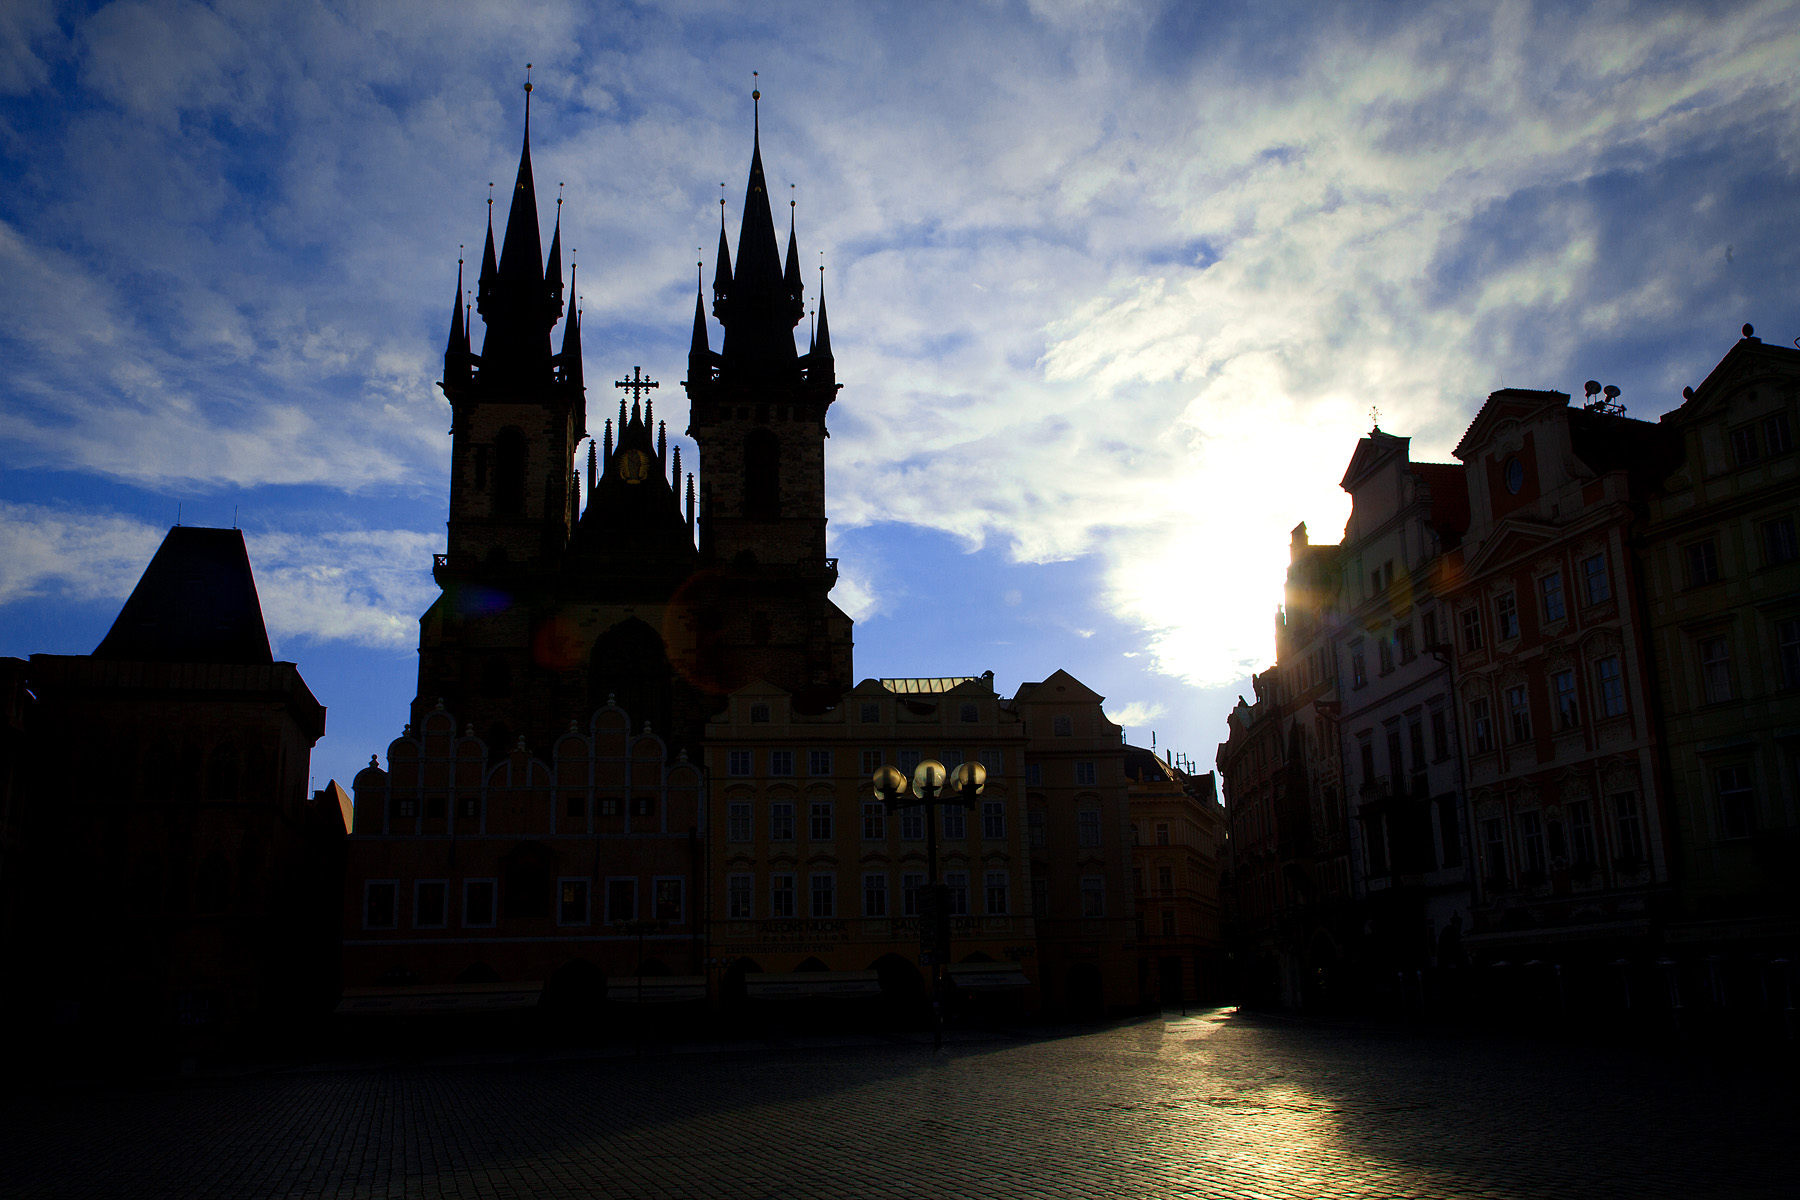
\includegraphics[width=8.5cm]{church.png}}
%  \vspace{2.0cm}
  \centerline{Test image for Histogram equalization\cite{WEBSITE:13}}\medskip
\end{minipage}
%
\end{figure}
This is image is chosen for histogram equalization because its Histogram is more skewed towards low intensity levels. Results of histogram equalisation will be clearly visible with this image.

\subsection{Gamma Correct}
\begin{figure}[htb]

\begin{minipage}[b]{1.0\linewidth}
  \centering
  \centerline{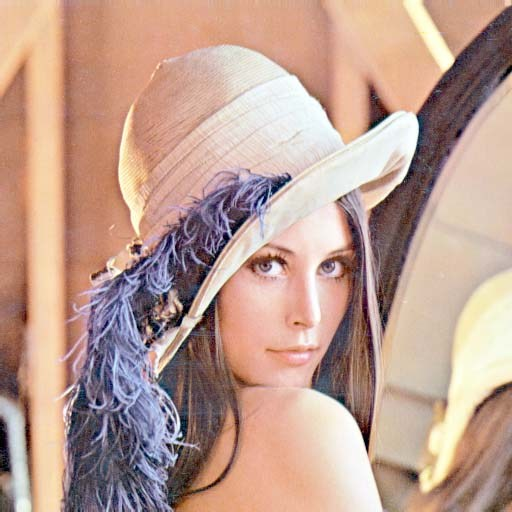
\includegraphics[width=8.5cm]{lena_gamhi.jpg}}
%  \vspace{2.0cm}
  \centerline{Test image for Gamma correction\cite{WEBSITE:12}}\medskip
\end{minipage}
%
\end{figure}
This is image is chosen for Gamma correction because it is brighter image and the effect of gamma transform for different gamma values can be clearly observed.

\subsection{Log Transform}
\begin{figure}[htb]

\begin{minipage}[b]{1.0\linewidth}
  \centering
  \centerline{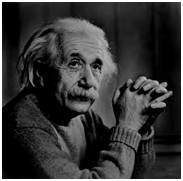
\includegraphics[width=8.5cm,height=7cm,keepaspectratio]{log_tst.jpg}}
%  \vspace{2.0cm}
  \centerline{Test image for Log Transform\cite{WEBSITE:16}}\medskip
\end{minipage}
%
\end{figure}
Effect of Log transformation is more clearly visible in Grey scale image, So grey scale image is chosen for testing Log transformation.

\subsection{Blur Image}
\begin{figure}[htb]

\begin{minipage}[b]{1.0\linewidth}
  \centering
  \centerline{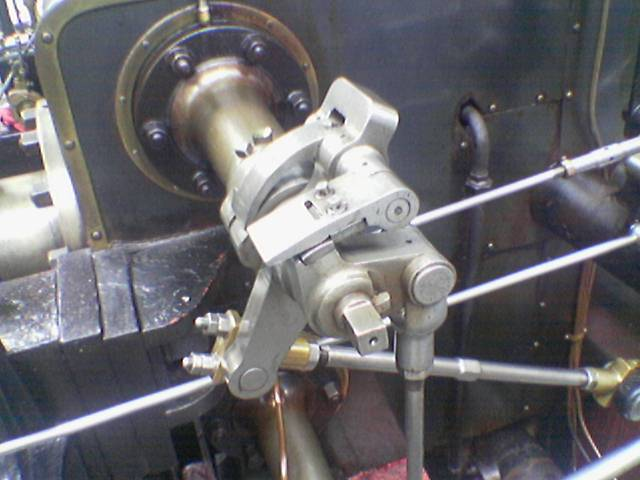
\includegraphics[width=8.5cm,height=5cm,keepaspectratio]{edges.png}}
%  \vspace{2.0cm}
  \centerline{Test image for Blurring\cite{WEBSITE:14}}\medskip
\end{minipage}
%
\end{figure}
Any image can chosen for blurring image but image which has more details in it will give the best output so this image is chosen.


\subsection{Sharpen Image}
\begin{figure}[htb]

\begin{minipage}[b]{1.0\linewidth}
  \centering
  \centerline{
\includegraphics[width=8.5cm,height=4cm,keepaspectratio]{done.jpg}}
%  \vspace{2.0cm}
  \centerline{Test image for Sharpening\cite{WEBSITE:17}}\medskip
\end{minipage}
%
\end{figure}


\subsection{Sobel operation}

\begin{figure}[htb]

\begin{minipage}[b]{1.0\linewidth}
  \centering
  \centerline{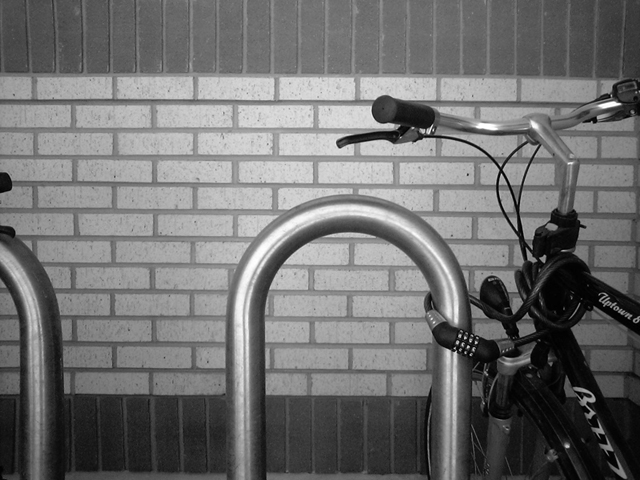
\includegraphics[width=8.5cm,height=5cm,keepaspectratio]{edge2.jpg}}
%  \vspace{2.0cm}
  \centerline{Test image for Sobel opeartion\cite{WEBSITE:15}}\medskip
\end{minipage}
%
\end{figure}
Image which has more horizontal and vertical edges will be required since Sobel operators for detecting horizontal and vertical edges is used as kernel

\section{Results on Test Images}
\label{sec:print}

Following are the images after appying various transformation techniques.
\subsection{Histogram Equalization}
\begin{figure}[htb]

\begin{minipage}[b]{1.0\linewidth}
  \centering
  \centerline{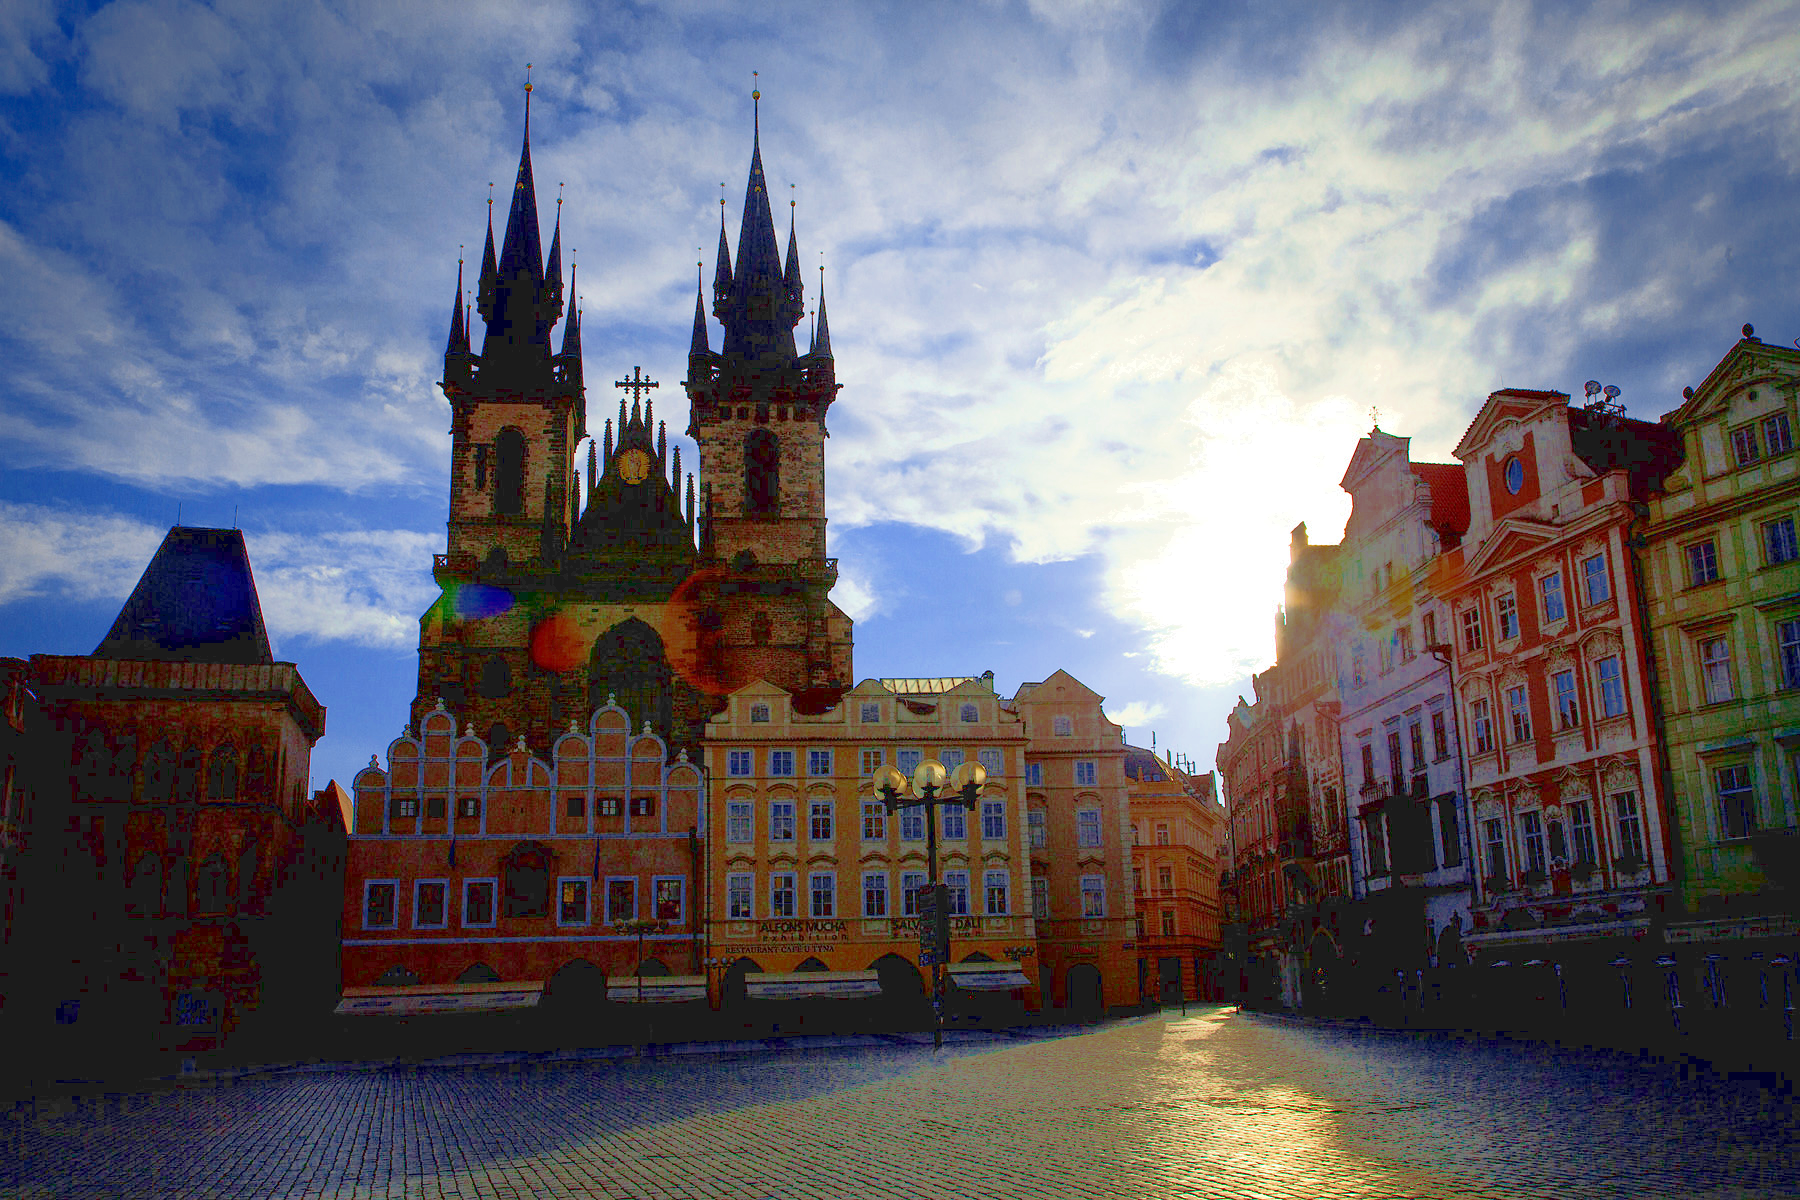
\includegraphics[width=8.5cm]{church_op.png}}
%  \vspace{2.0cm}
  \centerline{Test image after applying Histogram equalization}\medskip
\end{minipage}
%
\end{figure}


\subsection{Gamma Correct}
\subsubsection{gamma = 0.1}
\begin{figure}[htb]

\begin{minipage}[b]{1.0\linewidth}
  \centering
  \centerline{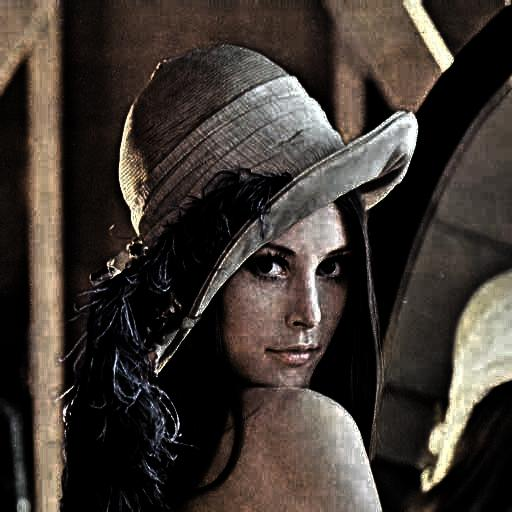
\includegraphics[width=8.5cm,height=6cm,keepaspectratio]{gamma0_1.jpg}}
%  \vspace{2.0cm}
  \centerline{Test image after applying Gamma correction with gamma = 0.1}\medskip
\end{minipage}
%
\end{figure}
\subsubsection[h]{gamma = 2.2}Image after applying gamma transform
\begin{figure}[h]

\begin{minipage}[b]{1.0\linewidth}
  \centering
  \centerline{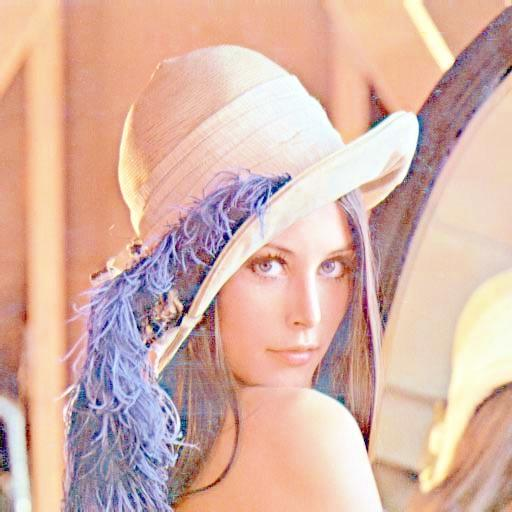
\includegraphics[width=8.5cm]{gamma2_2.jpg}}
%  \vspace{2.0cm}
  \centerline{Test image after applying Gamma correction with gamma = 2.2}\medskip
\end{minipage}
%
\end{figure}


\subsection[h]{Log Transform}
\begin{figure}[!h]

\begin{minipage}[b]{1.0\linewidth}
  \centering
  \centerline{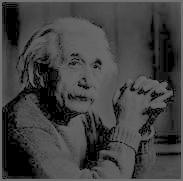
\includegraphics[width=8.5cm]{log_tst_op.jpg}}
%  \vspace{2.0cm}
  \centerline{Test image after applying Log Transform}\medskip
\end{minipage}
%
\end{figure}


\subsection[h]{Blur Image}Results of blurring with different Gaussian kernels
\subsubsection[h]{Blur using Gaussian kernel with variance 5 }
\begin{figure}[htb]

\begin{minipage}[b]{1.0\linewidth}
  \centering
  \centerline{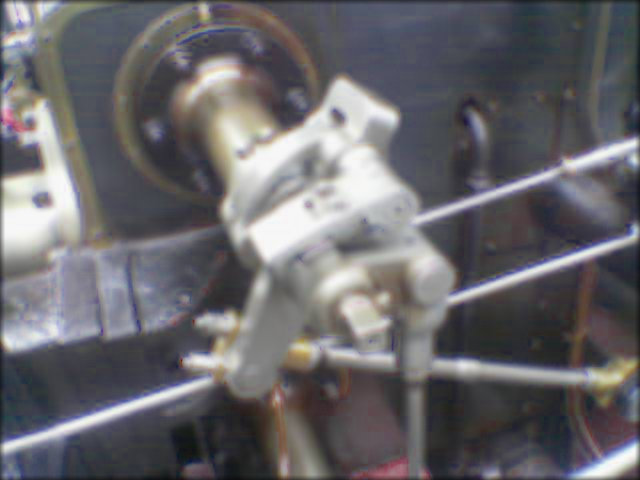
\includegraphics[width=8.5cm,height = 5cm ,keepaspectratio]{blur_5.png}}
%  \vspace{2.0cm}
  \centerline{Test image after Blurring with Gaussian kernel with variance 5}\medskip
\end{minipage}
%
\end{figure}
\subsubsection[h]{Blur using Gaussian kernel with variance 20}
\begin{figure}[h]

\begin{minipage}[b]{1.0\linewidth}
  \centering
  \centerline{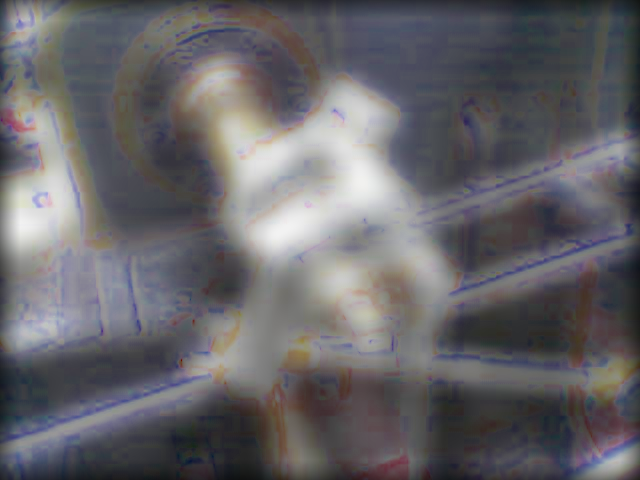
\includegraphics[width=8.5cm,height = 5cm ,keepaspectratio]{blur_20.png}}
%  \vspace{2.0cm}
  \centerline{Test image after Blurring with Gaussian kernel with variance 20}\medskip
\end{minipage}
%
\end{figure}


\subsection[h]{Sharpen Image}Result after applying Laplacian $(3,3)$ kernel
\begin{figure}[h]

\begin{minipage}[b]{1.0\linewidth}
  \centering
  \centerline{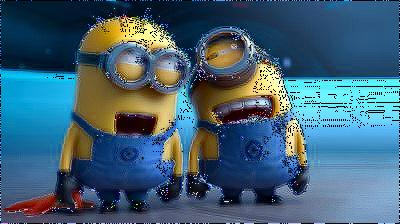
\includegraphics[width=8.5cm,height =4cm ,keepaspectratio]{done_op.jpg}}
%  \vspace{2.0cm}
  \centerline{Test image after applying sharpening filter}\medskip
\end{minipage}
%
\end{figure}


\subsection[h]{Sobel operation}Result of applying Sobel kernel to detect horizontal and vertical edges. Here the test image is convolved with the kernel to detect horizontal edges at the same time another kernel is applied to the test image to detect vertical edges to detect vertical edges. Result of the convolution of these is added to get the horizontal and vertical edges in image

\begin{figure}[htb]

\begin{minipage}[b]{1.0\linewidth}
  \centering
  \centerline{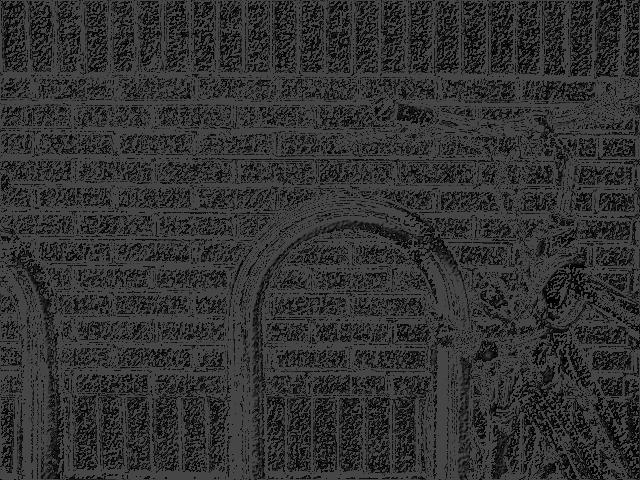
\includegraphics[width=8.5cm]{sobel_op.jpg}}
%  \vspace{2.0cm}
  \centerline{Test image after applying Sobel operator}\medskip
\end{minipage}
%
\end{figure}






\section{Disscussion}
\label{sec:ref}

Main problem faced during development is choice of language. I got to know that Matlab has a drag and drop type of making GUI, but it is licensed i wanted to work with open source. The choice I was left with was c++ and python. I was not well versed in both of them. Since python syntax is easy i chose python. Implementation of  GUI created a lot of problems I did not know which python binding to use, after searching online and found that tkinter is the basic and primitive binding in python so i chose that and started working with it but after spending entire day on it nothing much was happening so i shifted to pyqt after finding a tutorial\cite{WEBSITE:9} on pyqt and completed the GUI part using pyqt. For image operations Opencv \cite{WEBSITE:3}and numpy\cite{WEBSITE:1} libraries are used though it was not easy documentation is available online.

\\ If more time was given i would have implemented convolution using vectors to reduce the computations and GUI also can improved by  making the window responsive adding short cuts to all the operations etc.,

% References should be produced using the bibtex program from suitable
% BiBTeX files (here: strings, refs, manuals). The IEEEbib.bst bibliography
% style file from IEEE produces unsorted bibliography list.
% -------------------------------------------------------------------------
\bibliographystyle{IEEEbib}
\bibliography{strings,refs}
\onecolumn
\section{APPENDIX}
\subsection{Code using inbuilt FFT and IFFT functions }
\lstinputlisting[language=Python]{assignment2_1.py}
\subsection{Code  without using inbuilt FFT and IFFT functions }
\lstinputlisting[language=Python]{assignment2.py}
\end{document}
